\documentclass[a4paper]{article}

%% Language and font encodings
\usepackage[english]{babel}
\usepackage[utf8x]{inputenc}
\usepackage[T1]{fontenc}

%% Sets page size and margins
\usepackage[a4paper,top=3cm,bottom=2cm,left=3cm,right=3cm,marginparwidth=2cm]{geometry}

%% Useful packages
\usepackage{amsmath}
\usepackage{amsfonts}
\usepackage{bbm}
\usepackage{graphicx}
\usepackage[colorinlistoftodos]{todonotes}
\usepackage[colorlinks=true, allcolors=blue]{hyperref}
\usepackage{float}
\usepackage{enumerate}
\usepackage{mathrsfs}
\usepackage{caption}
\usepackage{subcaption}

\usepackage{pgfplots, pgfplotstable}
\pgfplotsset{compat=1.16}
\pgfplotsset{soldot/.style={color=blue,only marks,mark=*}} \pgfplotsset{holdot/.style={color=blue,fill=white,only marks,mark=*}}

\title{Stochastic Processes}
\author{Kevin Chang}

\graphicspath{ {./image/} }

\begin{document}
\maketitle

\section{}
\begin{itemize}
        \begin{figure} [H]
            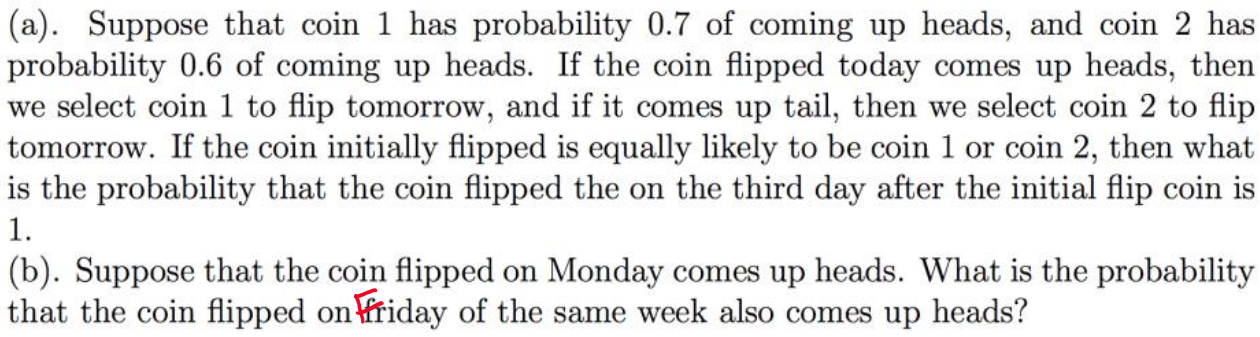
\includegraphics[width=1\linewidth]{image/1.png}
        \end{figure}
    \item $P = \left[ \begin{array}{cc} 0.7 & 0.3 \\ 0.6 & 0.4 \end{array} \right]$
    \item (a) $[0.5$ $0.5] P^3 = [0.6665$ $0.3335]$
    \item (b) $[1$ $0] P^3 = [0.6667$ $0.3333]$
\end{itemize}

\section{}
\begin{itemize}
        \begin{figure} [H]
            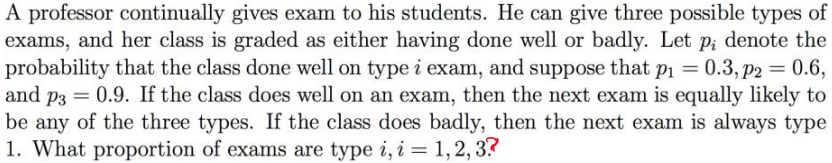
\includegraphics[width=1\linewidth]{image/2.png}
        \end{figure}
    \item $P = \left[ \begin{array}{ccc}
                0.8 & 0.1 & 0.1 \\
                0.6 & 0.2 & 0.2 \\
                0.4 & 0.3 & 0.3 \\
            \end{array} \right]$
    \item stationary distribution: $p$
        \begin{itemize}
            \item $p$ is eigenvector corresponding to eigenvalue 1 of $P^T$
            \item $p = [\frac{5}{7}$ $\frac{1}{7}$ $\frac{1}{7}]$
        \end{itemize}
\end{itemize}

\section{}
\begin{itemize}
        \begin{figure} [H]
            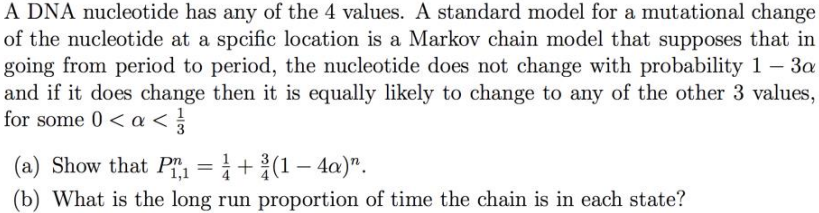
\includegraphics[width=1\linewidth]{image/3.png}
        \end{figure}
    \item $P = \left[ \begin{array}{cccc}
                1-3 \alpha & \alpha & \alpha & \alpha \\
                \alpha & 1-3 \alpha & \alpha & \alpha \\
                \alpha & \alpha & 1-3 \alpha & \alpha \\
                \alpha & \alpha & \alpha & 1-3 \alpha \\
            \end{array} \right]$
    \item (a)
        \begin{itemize}
            \item $P^n = \frac{1}{4}\left[ \begin{array}{cccc}
                        3(1-4\alpha)^n + 1 & 1 - (1-4\alpha)^n & 1 - (1-4\alpha)^n & 1 - (1-4\alpha)^n \\
                        1 - (1-4\alpha)^n & 3(1-4\alpha)^n + 1 & 1 - (1-4\alpha)^n & 1 - (1-4\alpha)^n \\
                        1 - (1-4\alpha)^n & 1 - (1-4\alpha)^n & 3(1-4\alpha)^n + 1 & 1 - (1-4\alpha)^n \\
                        1 - (1-4\alpha)^n & 1 - (1-4\alpha)^n & 1 - (1-4\alpha)^n & 3(1-4\alpha)^n + 1 \\
                \end{array} \right]$

                (by Wolfram Alpha)
            \item $P_{1, 1}^n = \frac{1}{4} + \frac{3}{4}(1-4\alpha)^n$
        \end{itemize}
    \item (b) it is equally distributed: stationary distribution is $\frac{1}{4}[1, 1, 1, 1]$
\end{itemize}

\section{}
\begin{itemize}
        \begin{figure} [H]
            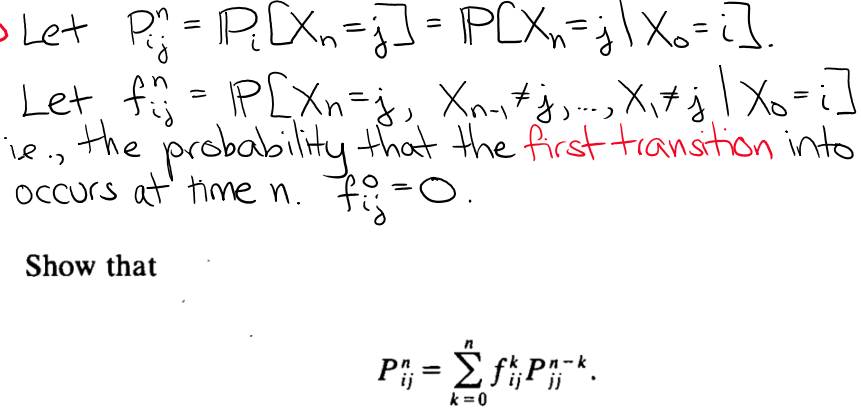
\includegraphics[width=1\linewidth]{image/4.png}
        \end{figure}
    \item $P_{ij}^n = P[X_n = j|X_0 = i] = P[X_n = j, X_1 = j|X_0=i] + P[X_n = j, X_1 \not = j|X_0=i]$

        $= P[X_n = j|X_1 = j, X_0=i]P[X_1=j|X_0=i] + P[X_n = j, X_1 \not = j|X_0=i]$

        $= P_{jj}^{n-1} f_{ij}^k + P[X_n = j, X_2 = j, X_1 \not = j|X_0=i] + P[X_n = j, X_2 \not = j, X_1 \not = j|X_0=i]$

        $= P_{jj}^{n-1} f_{ij}^2 + P_{jj}^{n-2} f_{ij}^2 + P[X_n = j, X_2 \not = j, X_1 \not = j|X_0=i]$

        $\dots$

        $= \sum_{k=0}^n P_{jj}^{n-k} f_{ij}^k$
\end{itemize}

\section{}
\begin{itemize}
        \begin{figure} [H]
            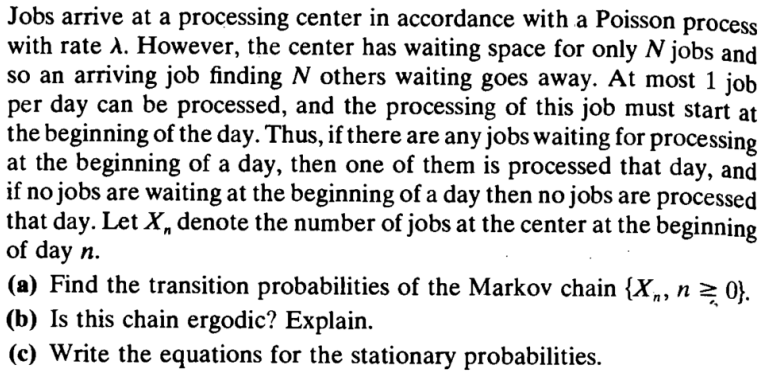
\includegraphics[width=1\linewidth]{image/5.png}
        \end{figure}
    \item $Y \sim$ Poisson($\lambda$)
    \item (a) $P = \left[ \begin{array}{ccccc}
                P[Y=0] & P[Y=1] & \dots & \dots & P[Y=N] \\
                P[Y=0] & P[Y=1] & \dots & \dots & P[Y=N] \\
                0 & P[Y=0] & P[Y=1] & \dots & P[Y\geq N-1] \\
                \dots & \dots & \dots & \dots & \dots \\
                0 & 0 & \dots & P[Y=1] & P[Y\geq 1] \\
            \end{array} \right]$
    \item (b) yes it is ergodic, since it is aperiodic and irreducible
\end{itemize}

\section{}
\begin{itemize}
        \begin{figure} [H]
            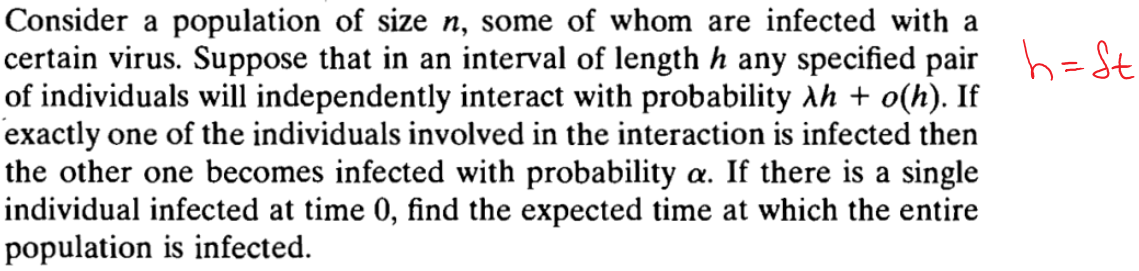
\includegraphics[width=1\linewidth]{image/6.png}
        \end{figure}
    \item $R = \left[ \begin{array}{cccccc}
                -\lambda & \lambda(1-\alpha) & \lambda \alpha & \dots & \dots & 0 \\
                0 & -\lambda & \lambda(1-\alpha) & \lambda \alpha & \dots & 0 \\
                \dots & \dots & \dots & \dots & \dots & \dots \\
                0 & \dots & \dots & \dots & \dots & 0 \\
            \end{array} \right]$
    \item Suppose
        \begin{itemize}
            \item $N$ is the number of infection
            \item $X_i$ is the number of infected perseon in each time
        \end{itemize}
    \item $\sum_{i=1}^N X_i - N \mathbb{E}[X_i]$ is a martingale
    \item $\mathbb{E}[N] = \frac{n-1}{\mathbb{E}[X_i]} = \frac{n-1}{1+a}$
    \item Expected time at which the whole population is infected: $\lambda \frac{n-1}{1+a}$
\end{itemize}

\section{}
\begin{itemize}
        \begin{figure} [H]
            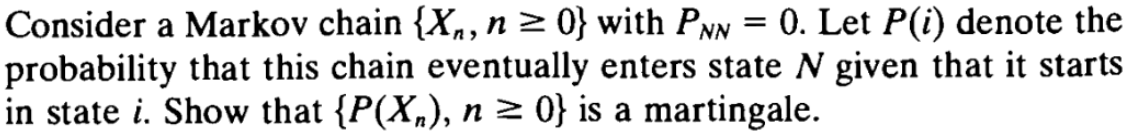
\includegraphics[width=1\linewidth]{image/7.png}
        \end{figure}
    \item $A$ is a random variale such that

        $A = \left\{ \begin{array}{cc} 1 & \text{if this chain eventually enters state $N$} \\ 0 & \text{otherwise} \end{array} \right.$
    \item $P(X_n) = \mathbb{E}[A|X_n]$
    \item $\mathbb{E}[P(X_{n+1})| X_n, \dots, X_1]$
        $= \mathbb{E}[\mathbb{E}[A|X_{n+1}]| X_n, \dots, X_1] = \mathbb{E}[A|X_n] = P(X_n)$
    \item $\mathbb{E}[P(X_n)] \leq 1$
\end{itemize}

\section{}
\begin{itemize}
        \begin{figure} [H]
            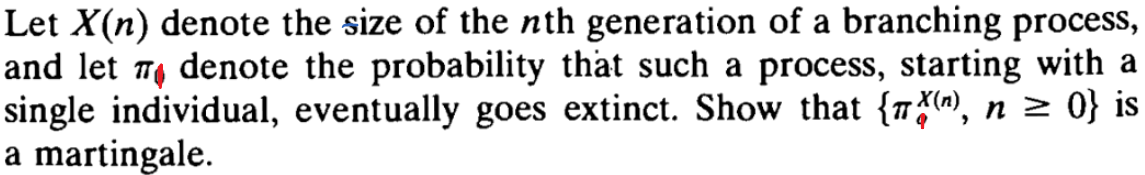
\includegraphics[width=1\linewidth]{image/8.png}
        \end{figure}
    \item $A$ is a random variale such that

        $A = \left\{ \begin{array}{cc} 1 & \text{if this chain eventually enters state $N$} \\ 0 & \text{otherwise} \end{array} \right.$
    \item $\pi^{X(n)} = \mathbb{E}[\pi|X(n), \dots, X(0)]$
    \item $\mathbb{E}[\pi^{X(n+1)}| X(n), \dots, X(0)]$
        $= \mathbb{E}[\mathbb{E}[\pi|X(n+1), X(n), \dots, X(0)]| X(n), \dots, X(0)]$

        $= \mathbb{E}[\pi|X(n), \dots, X(0)]$
        $= \pi^{X(n)}$
    \item $\mathbb{E}[\pi^{X(n)}| X(n-1), \dots, X(0)] \leq 1$
\end{itemize}

\section{}
\begin{itemize}
        \begin{figure} [H]
            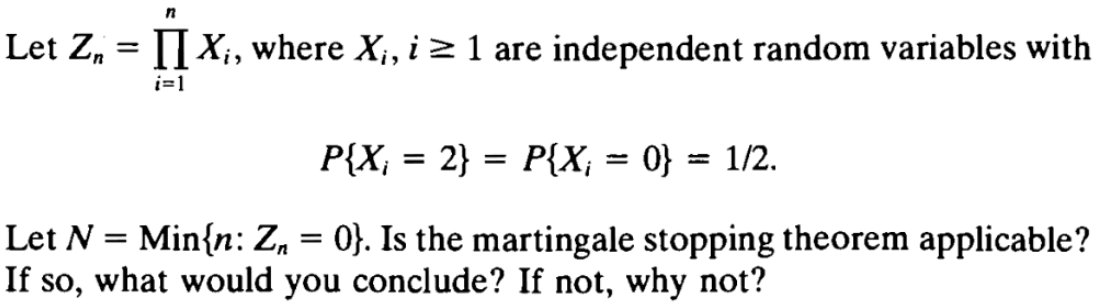
\includegraphics[width=1\linewidth]{image/9.png}
        \end{figure}
    \item No
        \begin{itemize}
            \item By first rule
                \begin{itemize}
                    \item We can not find a constant $k$ such that $P[N<k] = 1$
                \end{itemize}
            \item By second rule
                \begin{itemize}
                    \item We can not find a constant $k$ such that $P[\prod_{i=1}^n X_i < k] = 1$
                \end{itemize}
            \item By third rule
                \begin{itemize}
                    \item $\mathbb{E}[N] = \sum_{i=1}^\infty i 2^{-i} = 2$
                    \item We can not find a constant $k$ such that $\mathbb{E}[|Z_{n+1} - Z_n||Z_n, \dots, Z_1] = Z_n < k$
                \end{itemize}
        \end{itemize}
\end{itemize}

\section{}
\begin{itemize}
        \begin{figure} [H]
            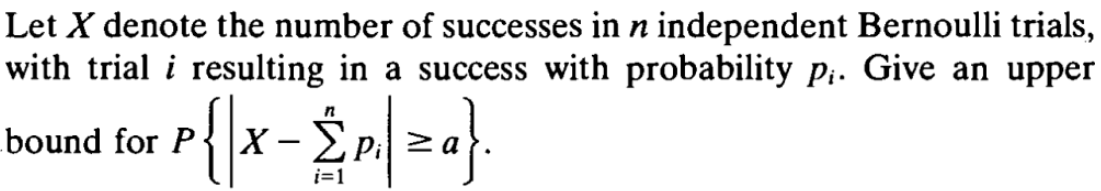
\includegraphics[width=1\linewidth]{image/10.png}
        \end{figure}
    \item $S_i$ $i$-th Bernoulli trial
    \item $Z_n = \sum_{i=1}^n S_i - \sum_{i=1}^n p_i$ is a martingale
        \begin{itemize}
            \item $\mathbb{E}[Z_n] < n$
            \item $\mathbb{E}[Z_{n+1}|S_n, \dots, S_1] = \mathbb{E}[Z_n + S_{n+1} - p_{n+1}|S_n, \dots, S_1] = Z_n$
        \end{itemize}
    \item By Azuma's inequality: $P[|Z_n| \geq a] \leq 2 e^{-\frac{a^2}{2n}}$
        \begin{itemize}
            \item $-1 \leq Z_{i+1} - Z_i \leq 1$
        \end{itemize}
\end{itemize}

\section{}
\begin{itemize}
        \begin{figure} [H]
            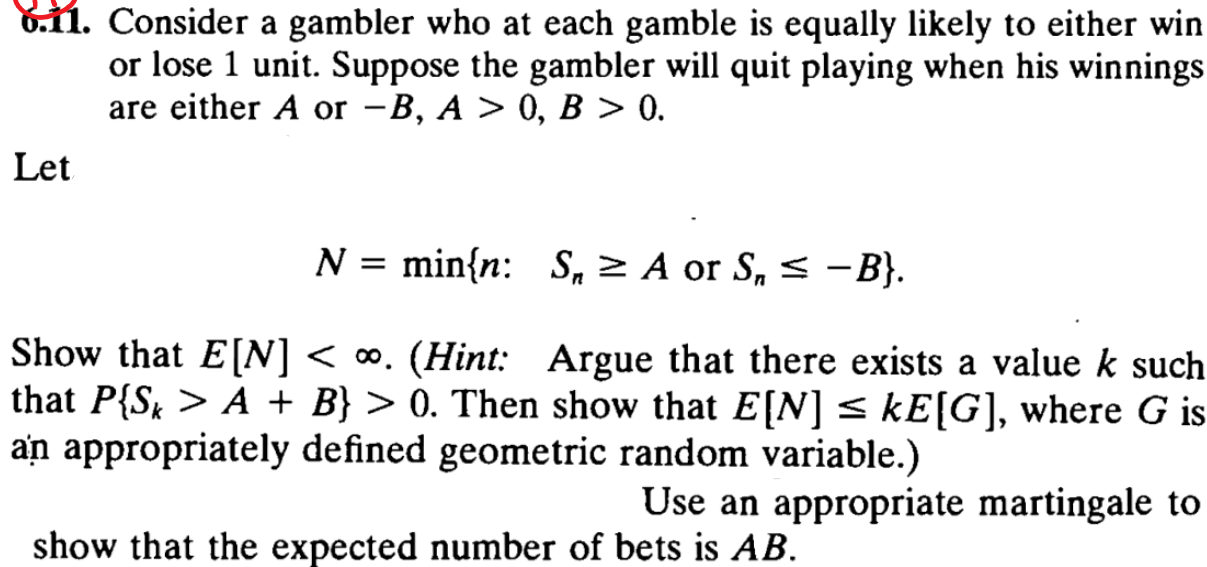
\includegraphics[width=1\linewidth]{image/11.png}
        \end{figure}
    \item $E$ is an event that the gambler wins successively $A+B$ times
    \item $P[E] = 2^{A+B}$
    \item $\mathbb{E}[\# \text{ of trials until } E] = \frac{1}{2^{A+B}}$
    \item $\mathbb{E}[N] \leq \frac{A+B}{2^{A+B}}$
    \item $Z_n = (\sum_{i=1}^n S_i)^2 - n$ is a martingale
        \begin{itemize}
            \item $\mathbb{E}[|Z_n|] < n^2$
            \item $\mathbb{E}[Z_{n+1}|S_n, \dots, S_1] = \mathbb{E}[Z_n + S_{n+1}^2 + 2S_{n+1}(\sum_{i=1}^n S_i) - 1|S_n, \dots, S_1] = Z_n$
        \end{itemize}
    \item By third rule
        \begin{itemize}
            \item $\mathbb{E}[N] \leq \infty$
            \item $\mathbb{E}[|Z_{n+1} - Z_n||Z_n, \dots, Z_1]$

                $= \mathbb{E}[|S_{n+1}^2 + 2S_{n+1}(\sum_{i=1}^n S_i) - 1||S_n, \dots, S_1] \leq 1 + 2(A+B) + 1$
        \end{itemize}
    \item $\mathbb{E}[Z_N] = 0$
        \begin{itemize}
            \item $\mathbb{E}[Z_N] = \mathbb{E}[(\sum_{i=1}^N S_i)^2] - \mathbb{E}[N] = 0$
            \item $\mathbb{E}[N] = \frac{A}{A+B}B^2 + \frac{B}{A+B}A^2 = AB$
        \end{itemize}
\end{itemize}

\section{}
\begin{itemize}
        \begin{figure} [H]
            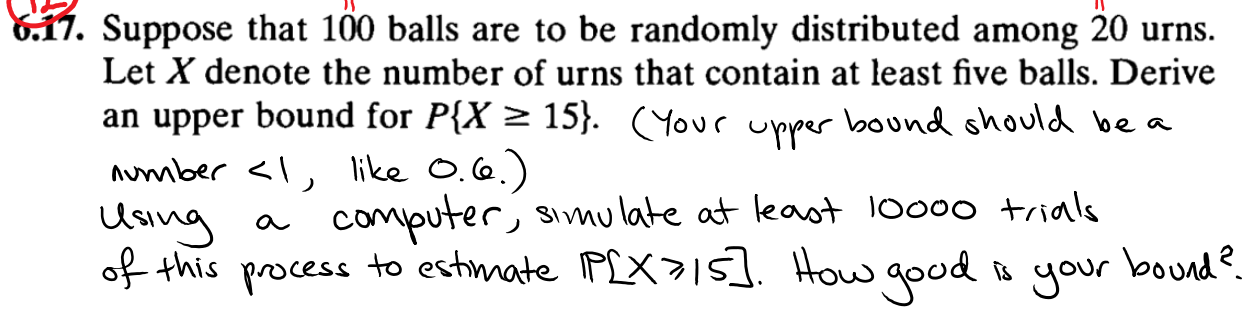
\includegraphics[width=1\linewidth]{image/12.png}
        \end{figure}
    \item $\mathbb{E}[X]$
        \begin{itemize}
            \item $\mathbb{E}[X] = 20 \times (1 - \frac{19^{100} + \binom{100}{1}19^{99} + \binom{100}{2}19^{98} + \binom{100}{3}19^{97} + \binom{100}{4}19^{96}}{20^{100}}) \approx 11.2803)$
        \end{itemize}
    \item $B_i$ is the result for $i$-th ball
    \item By Azuma's inequality: $P[|Z_n - \mathbb{E}[X]| \geq a] \leq 2 e^{-\frac{a^2}{2n}}$
        \begin{itemize}
            \item $P[|Z_n - \mathbb{E}[X]| \geq a] \leq 2 e^{-\frac{a^2}{2n}}$
            \item $P[X \geq 15] \leq 2 e^{-\frac{(15-\mathbb{E}[X])^2}{200}} \approx 0.93316$
        \end{itemize}
    \item Simulation
        \begin{figure} [H]
            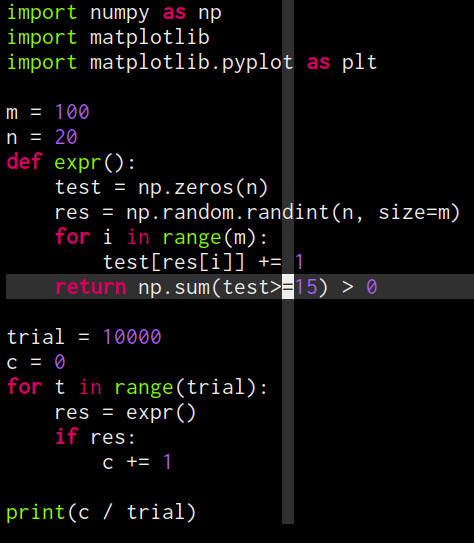
\includegraphics[width=0.5\linewidth]{image/code.png}
        \end{figure}
    \item Result
        \begin{figure} [H]
            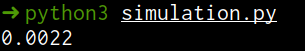
\includegraphics[width=0.5\linewidth]{image/result.png}
        \end{figure}
\end{itemize}

\end{document}
